\documentclass[a4paper,twocolumn,conference]{IEEEtran}


% *** GRAPHICS RELATED PACKAGES ***
%
\ifCLASSINFOpdf
   \usepackage[pdftex]{graphicx}
  % declare the path(s) where your graphic files are
   \graphicspath{{fig/}}
  % and their extensions so you won't have to specify these with
  % every instance of \includegraphics
  % \DeclareGraphicsExtensions{.pdf,.jpeg,.png}
\else
  % or other class option (dvipsone, dvipdf, if not using dvips). graphicx
  % will default to the driver specified in the system graphics.cfg if no
  % driver is specified.
  % \usepackage[dvips]{graphicx}
  % declare the path(s) where your graphic files are
  % \graphicspath{{../eps/}}
  % and their extensions so you won't have to specify these with
  % every instance of \includegraphics
  % \DeclareGraphicsExtensions{.eps}
\fi

\usepackage{multicol}
\usepackage{url}
\usepackage{graphicx}

%\hyphenation{net-works inter-domain}

\begin{document}

% paper title

\title{Cross-Layer Fault Management in Network Function Virtualization}

\author{\IEEEauthorblockN{Feng Liu}
	\IEEEauthorblockA{%Munich Network Management Team\\
		Huawei European Research Center\\
		Riesstr.25, M\"unchen, Germany}
%\and
}

\maketitle

\begin{abstract}
	Fault management (FM) play a vital role in the daily operation of teleco providers, however, we identify in
this paper that, Network Function Virtalization (NFV), despite its glorious technical advantages, aggravates
FM in multiple ways: \textit{first}, each abstraction layer has its own approaches to treat faults,
coordination between them is still a missing piece; \textit{secondly}, an effective FM system at each single
layer does not necessarily lead to an overall efficient FM system. A cross-layer FM system is therefore
needed. In this paper, we analyze in details the scenario, problems and challenges faced by constructing such
a system.        

\end{abstract}

\IEEEpeerreviewmaketitle

\section{Introduction}
	\label{intro}
Thank its flexibility which directly leads to significant savings on OPEX \&
CAPEX as well as its increased agility on service innovations, the concept of
NFV~\cite{nfv} has been prevailing recently among teleco service operators. The
fundamental idea behinds NFV is to build virtualized software network devices
based on the hypervisor and Commercial-Off-The-Shelf (COTS) hardware. The
infrastructure on which NFV is based is thus not built specifically for high
reliability and availability purposes; on the other hand, teleco services normally
requires five nines of availability which is about an annual outage time of 5
minutes. Providers are now facing with the dilemma: while enjoying high
flexibility and saving costs, they have to accept the risks of reliability. In
the context of NFV, \textit{faults have to be taken as facts rather than
exceptions}. Currently, this is also one of the major reasons which hold back
the teleco operators to adopt NFV system in their operational environment.

To tackle this dilemma, a highly efficient fault management system is needed to
deal with and compensate the un-reliable soft- and hardware systems.  As
prescribed by many literature on reliability and availability~\cite{depdef}, FM
including detection of system faults and toleration as well as isolation of
system anomalies. Finally impacted system should be recovered and services
restored in a timely manner. One may argue however that each layer involved in
the holistic NFV system already possesses its own mechanism to deal with fault,
however a fundamental question in this case one should rise: is it enough to
have a collection of individual FM systems to make a holistically efficient NFV
FM system? If not, what can be done about it? In this paper, we elaborate to
analyze and clarify the problematics.  The purpose of this paper is to identify
gaps and research challenges of building of highly efficient NFV FM system. This
paper is organized as follows: Section \ref{scenario} presents a typical NFV
scenario, on which our further discussions are based; in
Section~\ref{problemstatement} we make a in-depth analysis of the issues and
problems involved in FM of NVF and try to crystallize research challenges; in
Section~\ref{research} we discuss research issues and a roadmap to solve this
complex problem of cross-layer FM.  


\section{Scenario}
	\label{scenario}
\begin{figure}[ht]
	\centering
	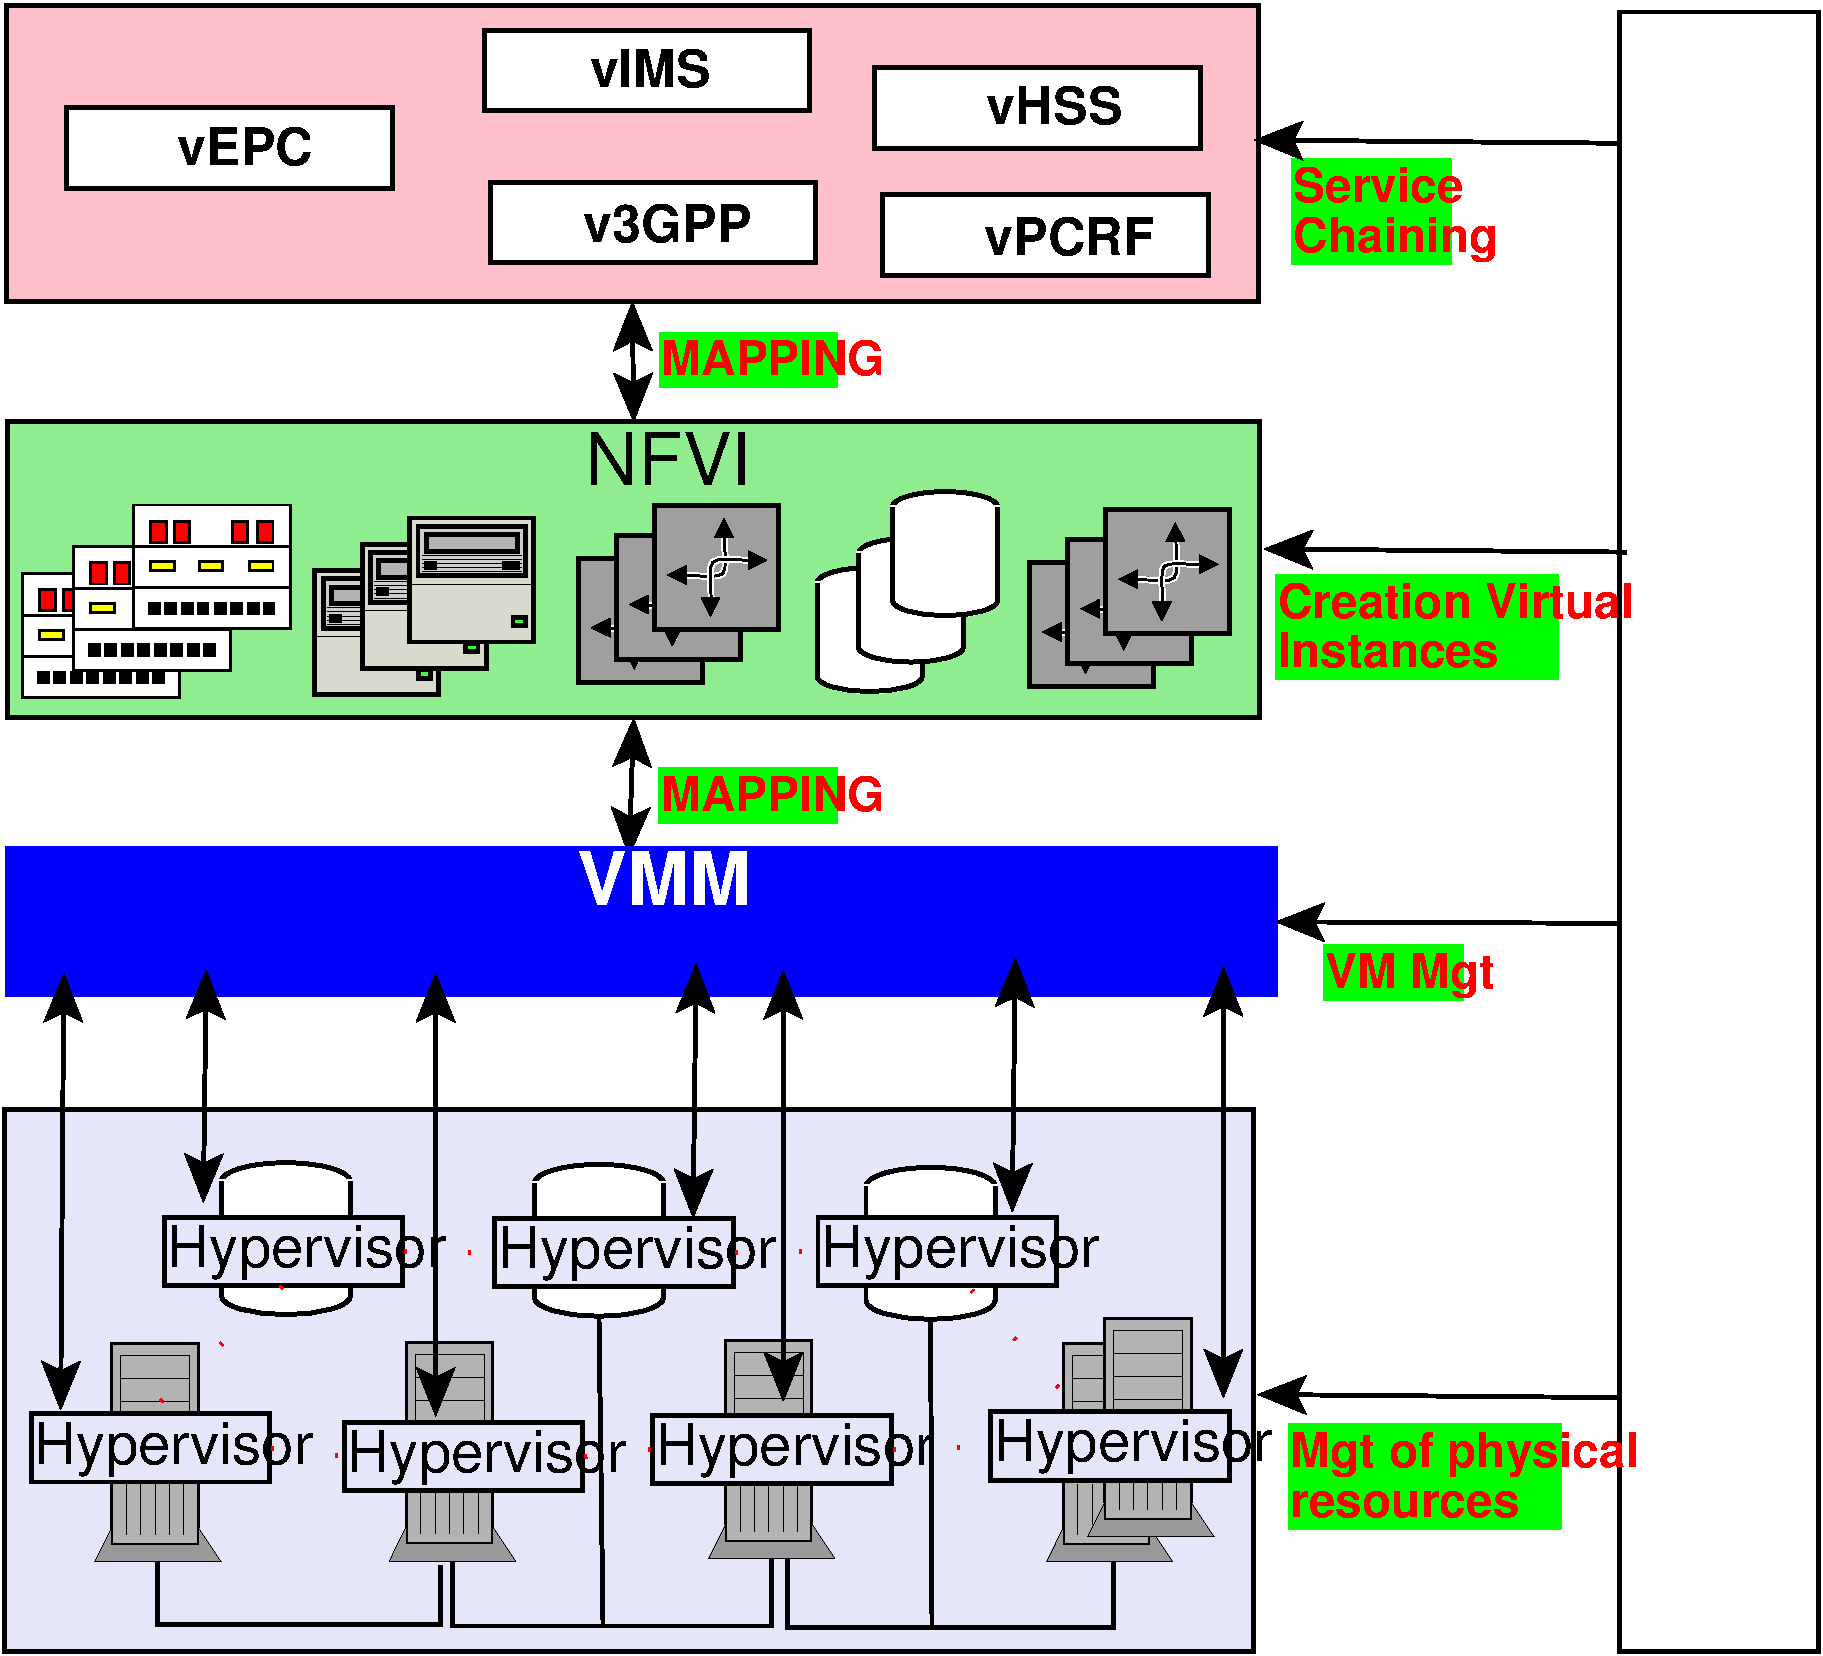
\includegraphics[scale=0.23]{fig/architecture-single.pdf}
	\caption{NFV Reference Architecture}
	\label{fig:arch}
\end{figure} 

In this discussion we use ETSI's NFV architectural model~\cite{nfv} as our main
reference model. Accordingly, the NFV architecture can be classified into three
layers: the first layer is comprised of hardware resources including computing,
storage and network devices, on which physical computing and communication take
place. Typically, this layer is built on computing clusters with
high-performance storage and networking devices. The second layer is
virtualization layer where one or more hypervisors virtualize hardware's
computing, communication and storage capabilities into sharable virtual
resources, some example of hypervisors suitable for such tasks are, KVM, Xen or
VMware, etc. Virtualization layer manages physical resources by means of
scheduling the usage of CPU cycle, network interface virtualization (vNIC) or
block storage devices through a pre-defined virtual infrastructure to hardware
interface (VI-Ha). Having the virtualization resources provisioned, virtual
infrastructures are now managed by platform such as OpenStack~\cite{openstack}
or CloudStack~\cite{cloudstack} for sharing among multiple tenants for service
implementation. A vertial component commonly known as Management and Netowork
Operation (MANO) is supposed to deal with management activities on different
layers and assist users to orchestrate NFV services on the top. 


%
\section{Problem Statement}
	\label{problemstatement}

\begin{table*}[!t]
\centering
\caption{Specific FM Approaches to Different NFV Layers}
\label{tbl:layers}
	\begin{tabular}{c|p{3cm}|p{5cm}}
		\hline
		\textbf{Layer} & \textbf{Typical HA Approaches} & \textbf{Example}\\
		\hline
		\hline
		Physical	&	Heartbeat, Fencing, Hot/Cold Standby, Reliable Messaging Bus &
LinuxHA Project, Pacemaker, cman \\
		Hypervisor & Virtual Resource Monitoring, Live Migration & VMWare HA, HA-Lizard \\
		Virtual Network Functions & Application-specific FM methods & vendor
specific application \\
		Virtual Services & Traditional Network Service OSS/BSS & SNMP or other
vendor specific methods to manage faults of virtual devices \\
\hline
	\end{tabular}
\end{table*} 
 
The central challenge in the cross-layer fault management lays in the coordination
of various FM appraoches from different layers involved in the NFV architecture
and, frequently, also within individual layers. We classify those problem in
\emph{vertical} and \emph{horizontal} dimensions. In this section, we analyze
research challenges in details accrodingly to the above mentioned dimensions,
then we provide a scenario that clarify an uncoordinated FM will aggreviate the
holistic system when failures impact. 

\subsection{Problems of Vertical Integration of FM Approaches} 

Typically each layer of NFV architecture possesses its own specific FM
approaches to ensure the services offered on this particular layer as we
illustrate in the Table~\ref{tbl:layers}. There is hardly any information
exchanged between layers regarding FM and let alone the coordination of
separated layers, let alone the coordinations among them. We argue that such a
separate approach does not meet requirements of a high efficient overall FM
system. Failing to do so will introduce various sorts of inconsistent problems
in terms of false positives in failure detections, inconsistent fault recovery
actions, which will only aggravate the holistic fault management process in general.

\subsubsection{Virtualization and Physical Layers}

Virtualization enables physical resources to be shared among multiple virtual
instances in terms of computing, networking and storage. While there are
different forms of resource virtualization, e.g. server, network, application
etc., different approaches have been applied to manage the virtual instances
which mostly concentrate on the efficient control of physical resources.
Features such as tracking of dependencies between virtual resources and their
physical mappings from service point of view is still missing piece.  Such kind
of dependency tracking is essential for the reliability both from top-down and
bottom-up perspective. When fault impacts virtualized resources, FM should
tracking down the associtated physical resources so that new resources could be
employed to mitgate faults and vice versa. This requires precise mappings
between layers since there could be one-to-many (aggregation) or many-to-one
(sharing) relationships between virtualized and physical resources. 
 
\subsubsection{NFVI and NFV Layers}

\subsubsection{FM by Orchestration of NFV Services}

\subsection{Problems of Horizontal Integration of FM Approaches}

\subsubsection{Coordinations between Distributed Clusters}

\subsubsection{Multi-Orchestrator Collaboration}


\section{Research Challenges}
	\label{research}


\section{Conclusion}
	\input{conclusion}

%\section*{Acknowledgment}

\bibliographystyle{IEEEtran}
\bibliography{clfman}

\end{document}
